% Overview:
%   FastGT TeX subfile for the project.
%   Each subfile MUST start with the following line
%		\documentclass[../main.tex]{subfiles}

\documentclass[../main.tex]{subfiles}

\begin{document}

\subsection{FastGT}
\label{fastgt}

FastGT \cite{pajuste2017fastgt} è un metodo computazionale che conta le frequenze di \textit{k}-mer unici nei dati delle read del genoma e utilizza queste informazioni per inferire i genotipi di varianti conosciute. È un tool molto veloce, in grado di rilevare le varianti in un genoma con coverage 30x in meno di 1 ora utilizzando un normale hardware a basso costo. Questo metodo fornisce un database di \textit{k}-mer che può poi essere utilizzato per la genotipizzazione simultanea di circa trenta milioni di SNV (Single-Nucleotide Variant), inclusi più di 23.000 SNV dal cromosoma Y. Attualmente FastGT utilizza solo regioni affidabili del genoma ed è limitato alla chiamata di varianti genomiche predefinite, non riesce a identificare varianti \textit{de novo}, poiché specifici \textit{k}-mer devono essere preselezionati per tutti gli alleli noti, ma non non si limita all'identificazione di SNV, può rilevare qualsiasi variante nota che può essere associata a un \textit{k}-mer unico e specifico per variante. È quindi ideale per una rapida analisi preliminare di un sottoinsieme di marcatori, successivamente seguita dall'analisi completa, quindi non sostituisce completamente la mappatura tradizionale e la chiamata di varianti ma è un metodo complementare che facilita alcuni aspetti delle analisi del genoma.

Il metodo si basa su tre componenti: (1) la procedura per la selezione di \textit{k}-mer unici, (2) la struttura dati personalizzata per l'archiviazione e il conteggio dei \textit{k}-mer direttamente da un file FASTQ\footnote{\ FastQ è un formato di puro testo in codice ASCII facilmente leggibile, pensato dal Wellcome Sanger Institute per associare ad una sequenza prodotta da una tecnologia NGS, la qualità di ogni sua singola base. È diventato lo standard de facto per la condivisione di dati \cite{cock2010sanger} \label{nota:FASTQ} prodotti da processi di sequenziamento basati su tecnologia NGS.} (vedi sezione \ref{AdaptiveRadixTree}) e (3) un modello probabilistico progettato per stimare i genotipi dai conteggi dei \textit{k}-mer.

\subsubsection{Adaptive Radix Tree}
\label{AdaptiveRadixTree}

L' Adaptive Radix Tree (ART) è una struttura dati progettata in \cite{leis2013art}, basata su \textit{trie}\footnote{\ Un \textit{trie} è una struttura dati ad albero ordinato usata per rappresentare un set, le cui chiavi sono tipicamente stringhe ordinate in ordine lessicografico; i nodi non conservano una copia della propria chiave, che dipende invece dalla posizione del nodo nell'albero. La radice è associata alla stringa vuota e tutti i discendenti di un nodo condividono il prefisso associato a quel nodo: attraversando l'albero si scende identificando la chiave parziale dei nodi. Le chiavi sono divise in chiavi parziali di \textit{s} bit ciascuna, dove \textit{s} è chiamato span: i nodi interni hanno 2\textit{s} puntatori figlio (possibilmente nulli), uno per ogni possibile sequenza \textit{s}-bit. Il vantaggio principale dei \textit{trie} rispetto all'hashing è l'ordinamento intrinseco.}, che riesce ad ottenere elevate prestazioni ed efficienza in termini di spazio, grazie alla compressione verticale e orizzontale dei nodi dell'albero. 

Per ottenere tali miglioramenti, il \textit{trie} viene \textit{adattato}. Normalmente, all'interno di un \textit{trie}, quando si memorizzano chiavi lunghe, si formano catene di nodi in cui ogni nodo ha un solo figlio sprecando spazio perciò, il primo ``adattamento" si ottiene comprimento verticalmente ciascun nodo senza fratelli al padre. Questo si può fare (1) in modo ``pessimistico", memorizzando una variabile aggiuntiva, il prefisso, all'interno di ciascun nodo che memorizza la concatenazione di chiavi parziali di discendenti che sono state eliminate perché non avevano fratelli, (2) in modo ``ottimista" memorizzando solo il numero di nodi compressi e nei nodi foglia le chiavi complete, oppure (3) in maniera ``ibrida", memorizzando il numero di nodi compressi e un array statico di dimensioni fisse per il percorso compresso.

Inoltre, con valori di span elevati, un \textit{trie} risulta essere molto schiacciato (in altezza) e con nodi molto grandi per i quali viene allocato molto spazio per i puntatori ai nodi figli, anche se non utilizzati. Per questa ragione, il secondo ``adattamento", riguardante la compressione orizzontale che \cite{leis2013art} propongono sono gli Adaptive Nodes, che utilizzano strutture dati dinamiche per tener conto dei figli, allocando meno spazio quando il numero di figli è piccolo. Un Adaptive Node, a seconda del numero di nodi figlio, si trova quindi tra quattro configurazioni, ottimizzate per un diverso numero di figli e adattate di conseguenza quando le chiavi vengono inserite o eliminate (ad esempio la configurazione più compatta, \texttt{Nodo4}, può avere fino a quattro figli). Ogni nodo presenta un'intestazione che memorizza il tipo di nodo, il numero di figli e la variabile prefisso, che contiene il percorso compresso (vedi \cite{leis2013art} per maggiori dettagli sulla struttura delle configurazioni). Infine, vengono utilizzate le  \textit{single-value leaves}, ovvero un tipo di nodo foglia aggiuntivo che memorizza un valore.

All'interno dell'ART si possono effettuare operazioni di ricerca, per controllare la presenza di un elemento confrontando le chiavi scendendo nell'albero e di eliminazione, nella quale il nodo foglia identificato dalla chiave di ricerca viene rimosso da un nodo interno, controllando poi se necessario applicare la compressione verticale ed inserzione.

Il consumo di spazio dell'ART dipende dalla distribuzione delle chiavi: chiavi dense rappresentano il caso migliore e possono essere archiviate in modo efficiente, anche utilizzando un intervallo ampio e senza nodi adattivi. Quando invece le chiavi sono sparse, molti puntatori di nodi interni sono nulli, il che si traduce in uno spazio sprecato. I nodi adattivi risolvono questi problemi e assicurano che qualsiasi distribuzione delle chiavi venga archiviata in modo compatto, ottimizzando localmente il consumo di spazio in ciascun nodo. Nel caso peggiore, tenendo conto dei nodi adattivi, della lenta espansione e della compressione del percorso, lo spazio occupato dai nodi dipende dalla loro tipologia e dal numero di figli.

\subsubsection{Struttura Dati}
\label{strutturaDatiFastGT}

L'input di FastGT è costituito da un file FASTQ contenente i dati del genoma e da un database precompilato di varianti genomiche e corrispondenti coppie di \textit{k}-mer che si sovrappongono a ciascuna variante. Ogni posizione bi-allelica del SNV nel genoma è coperta da \textit{k} coppie di \textit{k}-mer, dove la coppia è formata da \textit{k}-mer corrispondenti a due alleli alternati: si presuppone che almeno un numero di queste siano uniche e appaiano esclusivamente in una posizione del genoma; pertanto, i conteggi di occorrenze di queste coppie di \textit{k}-mer uniche nei dati di sequenziamento possono essere utilizzati per identificare il genotipo di questa variante in un individuo specifico. Sebbene una coppia di \textit{k}-mer sia teoricamente sufficiente per la genotipizzazione, le mutazioni occasionalmente cambiano la sequenza del genoma nelle vicinanze di un SNV, impedendone il rilevamento, rischiando di far dedurre il genotipo sbagliato: si utilizzano quindi fino a tre coppie di \textit{k}-mer per variante per prevenire chiamate errate causate da perdite occasionali di \textit{k}-mer a causa di rare mutazioni. FastGT utilizza una lunghezza \textit{k }= 25 dei \textit{k}-mer. \\

\noindent
FastGT utilizza un Adaptive Radix Tree (vedi Sezione \ref{AdaptiveRadixTree}) per memorizzare solo i \textit{k}-mer di interesse e i relativi conteggi, anziché tutti i possibili \textit{k}-mer del genoma. La struttura consente un buon compromesso tra il consumo di memoria e la velocità di ricerca. Infatti, data \textit{k} la lunghezza dei \textit{k}-mer inseriti nell'albero, nel caso peggiore sia le ricerche che le inserzioni nell'albero hanno complessità \textit{O}(log \textit{k}). I \textit{k}-mer sono codificati con 2 bit per nucleotide e memorizzati come stringhe di bit. I rami possono dividere la stringa sia tra diversi nucleotidi sia all'interno di un nucleotide. Il \textit{trie} è composto da numeri interi a 64 bit, ciascuno interpretato o come parte unica più a destra di un \textit{k}-mer (foglia) o come puntatore al ramo secondario successivo. L'albero non ha rami nel senso stretto del termine, ma i primi bit sono usati per selezionare il sottoalbero successivo. I nodi e le foglie sono interi a 64 bit. La Figura \ref{fig:art} è un esempio.

\begin{figure}[h!]
	\centering
  	\captionsetup{justification=centering}
  	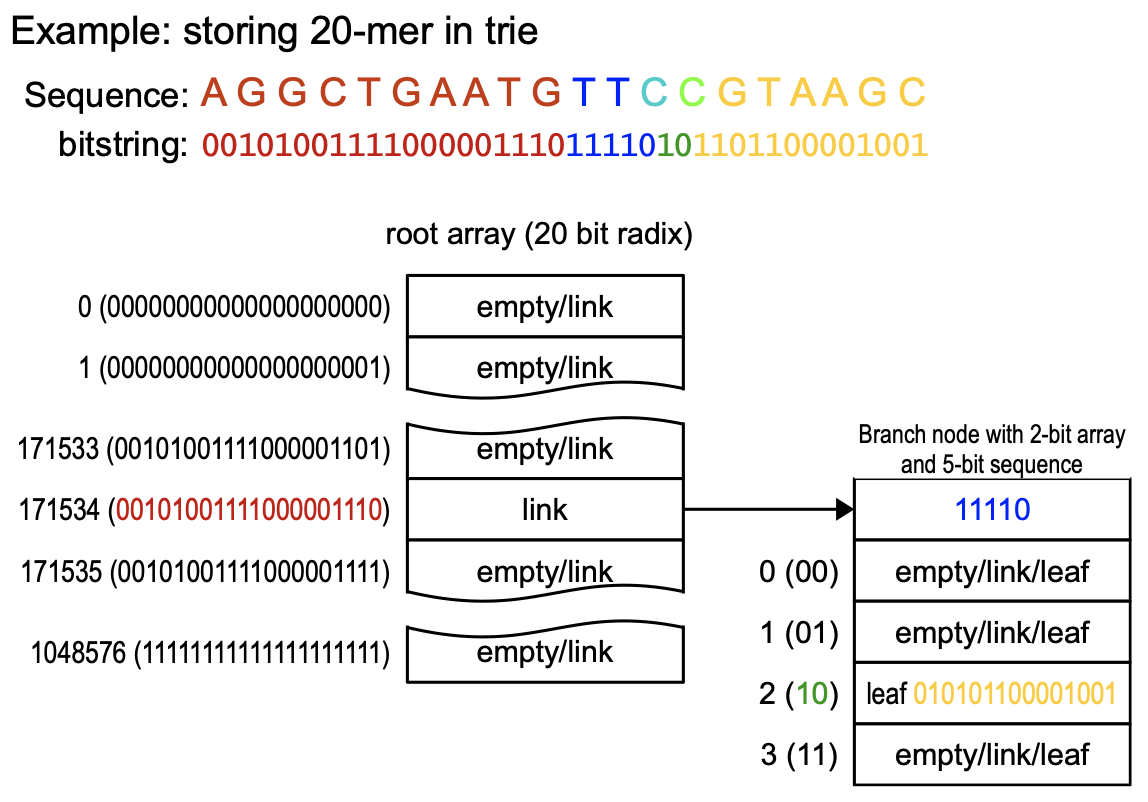
\includegraphics[scale=.35]{images/fastgt-art.png}
  	\caption{Layout semplificato dell'albero che memorizza 20-mer (40 bit), FastGT.}
  	\label{fig:art}
\end{figure}


\subsubsection{Algoritmo}

Il database delle varianti dei \textit{k}-mer univoci viene assemblato identificando tutte le possibili coppie di \textit{k}-mer per ogni variante, che poi vengono sottoposti a diversi passaggi di filtraggio. Le fasi di filtraggio rimuovono varianti per le quali non vengono osservati \textit{k}-mer unici e varianti che producono genotipi non canonici (non diploidi negli autosomi e non aploidi nei cromosomi X e Y maschili) in una serie di test sequenziati da individui. La procedura di filtraggio, che si può notare nella pipeline riportata in Figura \ref{fig:fastgt}, è la seguente:

 \begin{figure}[h!]
	\centering
  	\captionsetup{justification=centering}
  	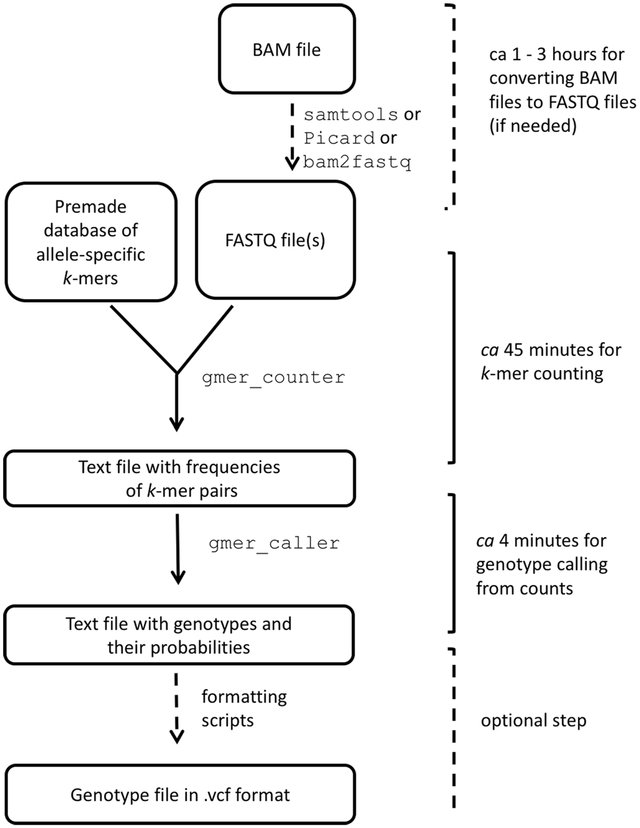
\includegraphics[scale=.25]{images/fastgt-pipeline.jpg}
  	\caption{Pipeline, FastGT.}
  	\label{fig:fastgt}
\end{figure}

\paragraph{Step 1} Partendo dagli SNV validati e gli indel comuni del database dbSNP (gli indel vengono usati solo per testare l'unicità dei \textit{k}-mer, non vengono inclusi nel database delle varianti), per ogni SNV bi-allelico vengono create due sequenze attorno alla posizione dell'SNV: quella del genoma di riferimento e quella corrispondente all'allele alternato. I \textit{k}-mer vengono filtrati e vengono eliminati i \textit{k}-mer che coprono un determinato SNV e che contengono altri SNV o indel noti, per rimuovere ogni possibile sovrapposizione: si vuole evitare di complicare gli algoritmi che effettuano il conteggio che altrimenti dovrebbero tener conto di molteplici combinazioni di alleli SNV vicini. 

\paragraph{Step 2} Viene testata l'unicità. Il parametro di unicità è esaminato rispetto al genoma di riferimento espanso, l'insieme dei 25-mer dal genoma di riferimento più tutti i possibili 25-mer contenenti gli alleli alternati. Una coppia di \textit{k}-mer è considerata unica se entrambi i \textit{k}-mer si verificano non più di una volta nel genoma di riferimento espanso: si rimuovono tutte le coppie non uniche.

\paragraph{Step 3} Infine, i \textit{k}-mer sono perfezionati testandone le frequenze, utilizzando le frequenze dei \textit{k}-mer e i genotipi in un set di genomi di 50 individui sequenziati\footnote{\ Il DNA dei 50 individui casuali utilizzati è stato raccolto e sequenziato durante il Center of Translational Genomics project presso l'Università di Tartu; vengono usati 25 uomini e 25 donne per filtrare gli SNV autosomici, 50 uomini per chrX e chrY. }. Vengono rimosse le coppie di \textit{k}-mer SNV con una frequenza anormalmente alta o un genotipo non canonico in più di un individuo. \\

\noindent
Dopo le fasi di filtraggio, nel test riportato in \cite{pajuste2017fastgt} dal database dbSNP sono rimasti utilizzabili 30 238 283 (64\%) SNV bi-allelici validati. Inoltre è stato usato un sottoinsieme di marcatori SNV autosomici presenti sul microarray Illumina HumanOmniExpress per un'analisi di concordanza.  \\

\noindent
La genotipizzazione viene eseguita leggendo le read non elaborate e contandone le frequenze delle coppie di \textit{k}-mer utilizzando il database precompilato delle varianti: si utilizzano i software personalizzati \texttt{gmer\_counter} e \texttt{gmer\_caller}. Le frequenze di \textit{k}-mer sono contate da \texttt{gmer\_counter}: si utilizza la struttura binaria degli adaptive radix tree per memorizzare sia le sequenze di \textit{k}-mer che le loro frequenze. Le frequenze di un massimo di tre coppie di \textit{k}-mer ottenute da \texttt{gmer\_counter} vengono salvate in un file di testo; infatti, per ridurre l'uso di \textit{k}-mer ridondanti, tra le coppie di \textit{k}-mer che si sovrappongono al SNV ne sono selezionate tre: si preferisce la coppia più a sinistra, la coppia più a destra e la coppia nel mezzo della regione, e se ciò non è possibile, perché una coppia non è univoca o contiene altri SNV, viene utilizzata la coppia \textit{k}-mer più lontana successiva. In questo modo se una rara mutazione su un lato dell'SNV cambia la sequenza su quel lato, ci si aspetta che la coppia dall'altro lato abbia ancora i conteggi previsti. Le frequenze di tutte e tre le coppie siano conteggiate da \texttt{gmer\_counter} ma successivamente \texttt{gmer\_caller} utilizza solo la coppia con un conteggio di frequenza totale più vicino alla frequenza media in un dato individuo. Il file di testo in output viene utilizzato da \texttt{gmer\_caller} che determina i genotipi in base alle frequenze e stampa i risultati su un altro file di testo. 

\texttt{gmer\_caller} utilizza il teorema Bayes per chiamare i genotipi a partire dalle frequenze dei \textit{k}-mer, calcolando la probabilità di ciascun genotipo e assegnando a ciascuna variante il genotipo più probabile. Le distribuzioni di frequenza degli alleli (di riferimento e alternativi) sono modellate da una distribuzione binomiale negativa con media uguale al prodotto della coverage e la vera molteplicità del \textit{k}-mer nel genoma; il modello consente di stimare il numero di copie più probabile per entrambi gli alleli. 

%\textcolor{red}{Infine, il genere dell'individuo viene determinato automaticamente dai dati di sequenziamento utilizzando, la frequenza media dei marker dal cromosoma X (chrX): se l'individuo è femmina, nel processo di chiamata viene utilizzato solo il modello autosomico (per chiamare gli SNV sia negli autosomi che nel cromosoma X) e non vengono chiamati i marcatori del cromosoma Y (chrY), per gli uomini un ulteriore modello aploide del classificatore di Bayes è addestrato per chiamare i genotipi degli SNV negli autosomi e anche nei cromosomi sessuali.}

\end{document}